\subsection{Experiment on Residue Correlation}
\label{subsec:exp:res}
\textbf{Inputs:}\\
We input a set of point clouds with the points consistently indexed respecting to their groundtruth correspondence, as shown in Figure~\ref{fig:input_for_exp_res}.\\
\begin{figure*}
	\centering
	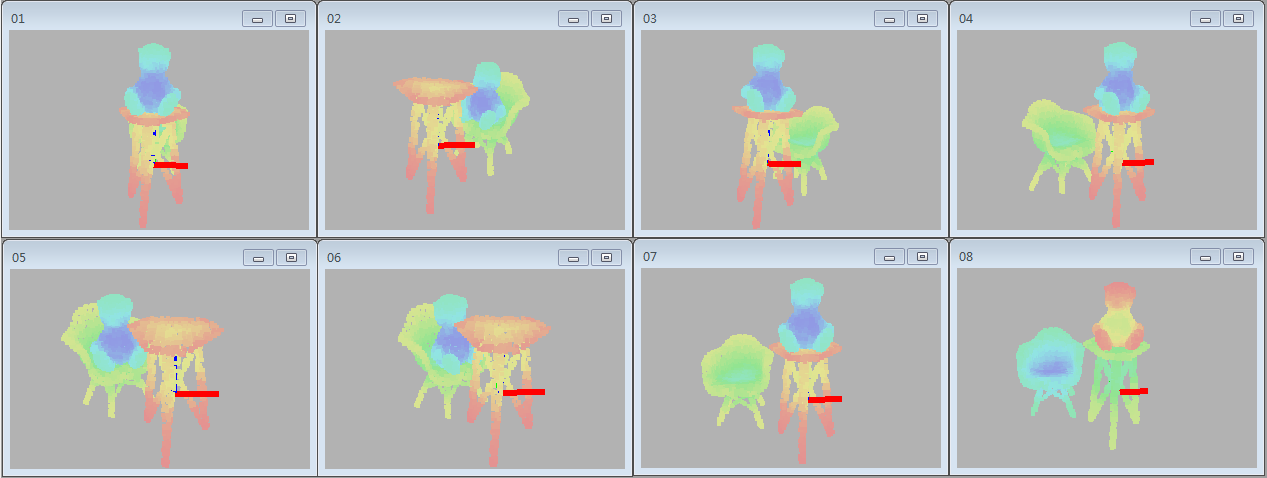
\includegraphics[width=\textwidth]{images/exp_res/inputs.png}
	\caption{Input of Experiment on Residue Correlation: The points are colored by their index. From the color you should be able to see that: In frame 01 - 07, the points are indexed consistently respecting to object in order of table, chair, teddy. In the frame 08, the points are indexed respecting to object in order of teddy, table, chair.}
	\label{fig:input_for_exp_res}
\end{figure*}
\textbf{Spectral Analysis:}\\
In order to do spectral analysis on point clouds, we first build supervoxels with \cite{Supervoxels} on point cloud and then construct a graph laplacian as a matrix $L=(a_{ij})$ defined by:
$$ a_{ij}=\left\{
\begin{aligned}
-\lambda d_{ij}-(1-\lambda) c_{ij} &~&if~i~and~j~is~an~edge\\
\sum\lambda d_{ij}+(1-\lambda) c_{ij} &~&if~i==j\\
0 &~&otherwise
\end{aligned}
\right.
$$
where $d_{ij}$
